\documentclass{beamer}
\usetheme{Warsaw}

\usepackage[utf8]{inputenc}
\usepackage{fancybox}
\usepackage{multimedia} 
\usepackage{subfig}
\usepackage{amsmath}
\usepackage{hyperref}
\hypersetup{
    colorlinks=true,     
    urlcolor=blue
}
\usepackage[all]{xy}

\setbeamertemplate{footline}[frame number]


\begin{document}


\title[Stochastik] % (optional, only for long titles)
{Wahrscheinlichkeitstheorie und Statistik (Stochastik)
\\
\includegraphics[scale=0.5]{img/craps}
}
\subtitle{}
\author[Dr. Johannes Riesterer] % (optional, for multiple authors)
{Dr.  rer. nat. Johannes Riesterer}

\date[KPT 2004] % (optional)
{}

\subject{Stochastik}

\frame{\titlepage}



\begin{frame}
    \frametitle{Diskrete Wahrscheinlichkeitsverteilung}
\framesubtitle{}

\begin{block}{Beispiel: Hash Kollision}

Beim Hashing werden zufällig $k$ Daten auf $n$ Speicherplätze  verteilt. Bezeichnen wir mit $A_{k,n}$ die Möglichkeiten der Mehrfachbelegungen von Feldern, so ist das komplementäre Ereignis
$A^c_{k,n} = Var^n_k(\Omega, o.W.)$,  wobei $\Omega$ die Menge der verfügbaren Speicherplätze darstellt. 
\end{block}


\begin{figure}[htp]
      \centering
    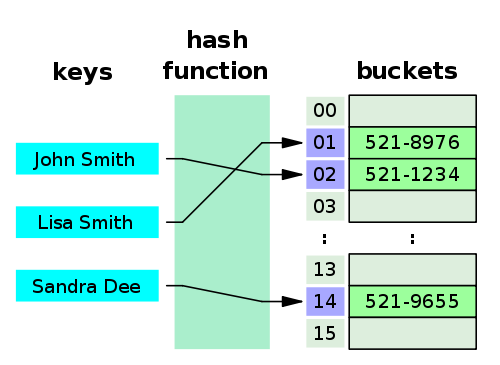
\includegraphics[width=0.5\textwidth]{img/hashtable}

      \caption{Quelle: Wikipedia}
\end{figure}


 \end{frame}


\begin{frame}
    \frametitle{Diskrete Wahrscheinlichkeitsverteilung}
\framesubtitle{}

\begin{block}{Beispiel: Hash Kollision}
\begin{align*}
 P(A^c_{k,n} ) & = \frac{\# Var^n_k(\Omega, o.W.)}{ \# Var^n_k(\Omega, m.W.)} = \\
 & \frac{n_k}{n^k} = \frac{n \cdot (n-1) \cdots (n-(k -1))}{n^k} = \prod_{i=0}^{k-1} (1- \frac{i}{n}) \\
& = \exp (\sum_{i=0}^{k-1} \ln {(1- \frac{i}{n})}) \leq  \exp (\sum_{i=0}^{k-1} (- \frac{i}{n})) \\
 & (ln(1-x) \leq -x \text{ für } x < 1) \\
&= \exp(- \frac{(k-1)k } {2n})
\end{align*}
\end{block}



 \end{frame}

\begin{frame}
    \frametitle{Diskrete Wahrscheinlichkeitsverteilung}
\framesubtitle{}

\begin{block}{Beispiel: Hash Kollision (Geburtstags-Paradoxon)}
Für $n=365$ und $k=23$ ist damit $ P(A_{k,n} ) > \frac{1}{2}$. Die Wahrscheinlichkeit, dass bei einer Gruppe von mehr als $23$ Leuten zwei Leute am gleichen Tag Geburtstag haben, ist also größer als $ \frac{1}{2}$.
\end{block}



 \end{frame}


\begin{frame}
    \frametitle{Diskrete Wahrscheinlichkeitsverteilung}
\framesubtitle{}

\begin{block}{Satz der totalen Wahrscheinlichkeit}
Für eine Zerlegung  $\Omega = \bigcup_{j=1}^{n} B_j, \text{ mit } B_i \cap B_k = \emptyset \text{ für } i \neq k $
\begin{align*}
& P(A ) = \sum_{j=1}^{n}  P(A \; | \;  B_j) \cdot P(B_j)
\end{align*}
\end{block}

 \end{frame}



\begin{frame}
    \frametitle{Diskrete Wahrscheinlichkeitsverteilung}
\framesubtitle{}

\begin{block}{Satz von Bayes}
Für $A,B \in \mathcal{A}$ mit  $P(B) > 0$ gilt
\begin{align*}
& P(A \; | \;  B) = \frac{P(B \; | \; A) \cdot P(A)} {P(B)} \\
\end{align*}
\end{block}

\begin{block}{Beweis}
\begin{align*}
& P(A \; | \;  B) =\frac{P(A \cap B)}{P(B)} = \frac{ \frac{P(A \cap B) \cdot P(A)}{P(A)}}{P(B)}  =  \frac{P(B \; | \; A) \cdot P(A)} {P(B)} 
\end{align*}
\end{block}



 \end{frame}



\begin{frame}
    \frametitle{Diskrete Wahrscheinlichkeitsverteilung}
\framesubtitle{}

\begin{block}{Erinnerung Stochastische Unabhängigkeit}
Zwei Ereignisse $A,B$ heißen stochastisch unabhängig, falls
\begin{align*}
P(A \cap B) = P(A) \cdot P(B)
\end{align*}
gilt.  Gleichbedeutend damit ist  $P(A | B) = P(A)$ und $P(B  | A) = P(B)$.
\end{block}

 \end{frame}


\begin{frame}
    \frametitle{Diskrete Wahrscheinlichkeitsverteilung}
\framesubtitle{}

\begin{block}{Naiver Bayes'scher Spam Filter}
Gegeben ist eine E-Mail $E$.  Wir möchten anhand des Vorkommens bestimmter Wörter $A_1, \ldots A_n$ in der Mail entscheiden, ob es sich um eine erwünschte Mail $H$ oder eine unerwünschte Mail $S$ (Ham or Spam) handelt. 
(Typische Wörter wären zum Beispiel "reich",  "casino", "Vergrösserung" ...)
\end{block}

\begin{figure}[htp]
      \centering
    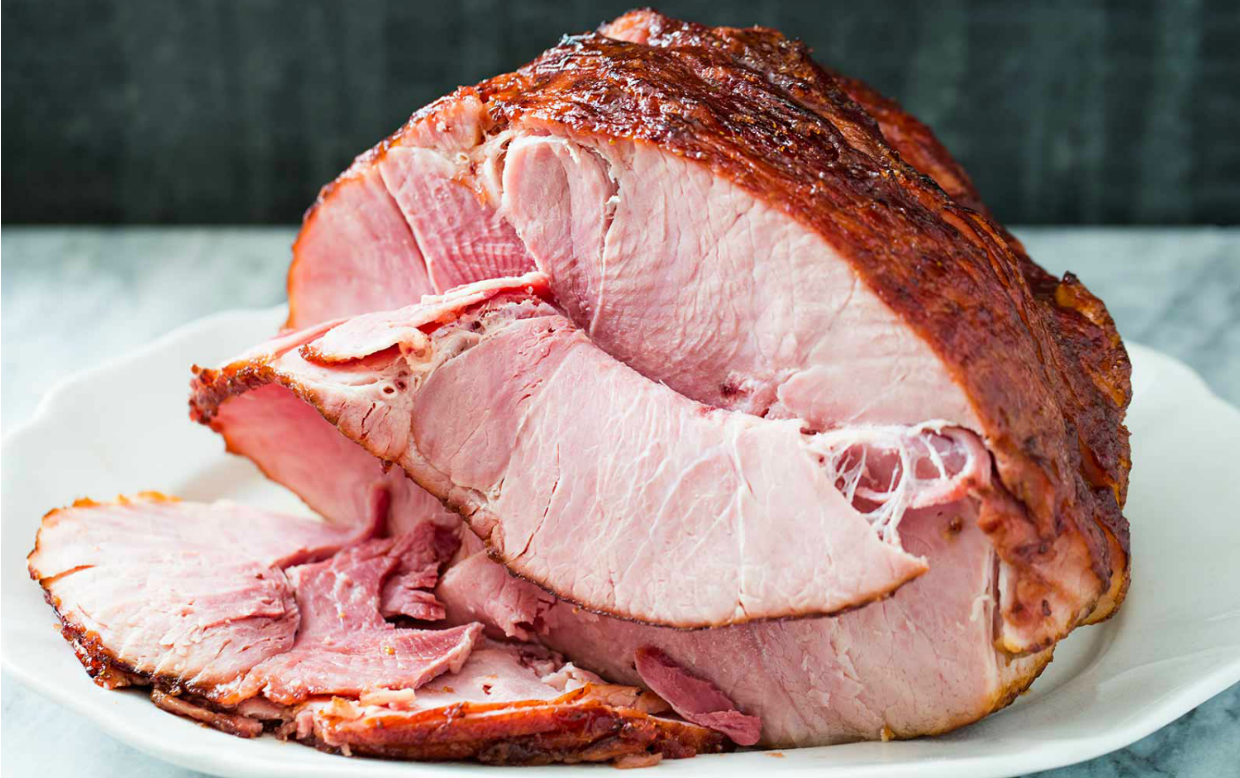
\includegraphics[width=0.4\textwidth]{img/ham}
    
\includegraphics[width=0.4\textwidth]{img/spam}

\end{figure}



 \end{frame}


\begin{frame}
    \frametitle{Diskrete Wahrscheinlichkeitsverteilung}
\framesubtitle{}

\begin{block}{Naiver Bayes'scher Spam Filter}

Aus einer Datenbank kann man das Vorkommen dieser Wörter in Spam und Ham Mails zählen und damit empirisch die Wahrscheinlichkeiten $P(A_i | S)$ und $P(A_i | H) $ des Vorkommens dieser Wörter in Spam und Ham Mails ermitteln.  Wir gehen davon aus, dass es sich bei der Mail  prinzipiell mit  Wahrscheinlichkeit $P(E= S) = P(E= H)= \frac{1}{2}$  um eine erwünschte  Mail $H$ oder eine unerwünschte Mail $S$  handeln kann. 
\end{block}

 \end{frame}



\begin{frame}
    \frametitle{Diskrete Wahrscheinlichkeitsverteilung}
\framesubtitle{}

\begin{block}{Naiver Bayes'scher Spam Filter}
 Wir machen zudem die (naive) Annahme, dass das Vorkommen der Wörter  stochastisch unabhängig ist, also 
\begin{align*}
P(A_1 \cap \cdots \cap A_n | S) = P(A_1 | S) \cdot P(A_2 | S) \cdots P(A_n | S) \\
P(A_1 \cap \cdots \cap A_n | H) = P(A_1 | H) \cdot P(A_2 | H) \cdots P(A_n | H)
\end{align*}
gilt.
\end{block}

 \end{frame}


\begin{frame}
    \frametitle{Diskrete Wahrscheinlichkeitsverteilung}
\framesubtitle{}

\begin{block}{Naiver Bayes'scher Spam Filter}
Mit der Formel von Bayes, der totalen Wahrscheinlichkeit  und kürzen, da $P(S) = P(H)$ können wir somit berechnen
\begin{align*}
& P(E=S |  A_1 \cap \cdots \cap A_n) = \frac{P(A_1 \cap \cdots \cap A_n | S) \cdot P(S)}{P(A_1 \cap \cdots \cap A_n)} \\
&=  \frac{P(A_1 | S) \cdots P(A_n | S) }{P(A_1 \cap \cdots \cap A_n | H) + P(A_1 \cap \cdots \cap A_n | S)} \\
&=  \frac{P(A_1 | S) \cdots P(A_n | S) }{P(A_1 | H) \cdots P(A_n | H)  + P(A_1 | S) \cdots P(A_n | S) } \\
\end{align*}
Bemerkung: $P(E=H |  A_1 \cap \cdots \cap A_n) = 1- P(E=S |  A_1 \cap \cdots \cap A_n) $
\end{block}



 \end{frame}





 \begin{frame}
    \frametitle{Erwartungswert}
\framesubtitle{}
\begin{block}{Eigenschaften}
Sind $X,Y : \Omega \to \mathbb{R}^n$   reelle, integrierbare  Zufallsvariablen und $a,b \in \mathbb{R}$ konstant, so gilt:
\begin{align*}
& \mathbb{E}(a \cdot X + b \cdot Y) = a \cdot \mathbb{E}(X) + b \cdot \mathbb{E}(Y) \\
& X(x) \leq Y(x) \;  \forall x \in \Omega \Rightarrow \mathbb{E}(X) \leq \mathbb{E}(Y) \\
& X ,Y \text{ stoch. unabhängig} \Rightarrow   \mathbb{E}(X \cdot Y) =  \mathbb{E}(X) \cdot  \mathbb{E}(Y) \\
& \mathbb{E} (1_A) = P (A)
\end{align*}
\end{block}
 \end{frame}

 \begin{frame}
    \frametitle{Erwartungswert}
\framesubtitle{}
\begin{block}{Varianz}
Für eine reelle Zufallsvariable ist die Varianz definiert durch
$$ \mathbb{V} (X) :=  \mathbb{E}( (X - \mathbb{E}(X))^2) \; .$$
\end{block}
\begin{block}{Verschiebungssatz}

\begin{align*}
 \mathbb{V}(X) & = \mathbb{E}(X^2 - 2X \mathbb{E}(X) + \mathbb{E}(X)^2) = \mathbb{E}(X^2) - 2 \mathbb{E}(X)^2 +  \mathbb{E}(X)^2 \\
& =  \mathbb{E}(X^2) -  \mathbb{E}(X)^2 \\
\end{align*}
\end{block}
 \end{frame}

 \begin{frame}
    \frametitle{Erwartungswert}
\framesubtitle{}
\begin{block}{Kovarianz}
Für  reelle Zufallsvariable $X,Y$ ist die Kovarianz definiert durch
$$ \mathcal{C} (X,Y) :=  \mathbb{E}( (X - \mathbb{E}(X)) (Y - \mathbb{E}(Y))) \; .$$
\end{block}

\begin{block}{Kovarianz}
    Per Definition ist
    $$ \mathcal{C} (X,X) :=  \mathbb{V}(X).$$
    \end{block}
 \end{frame}



\begin{frame}
    \frametitle{Erwartungswert}
\framesubtitle{}
\begin{block}{Beispiel}
$\Omega = \{ \text{Kopf},\text{Zahl}\}$, $P(\text{Kopf}) = P(\text{Zahl}) = \frac{1}{2}$, $X(\text{Kopf}) = 0,  X(\text{Zahl}) = 1$ 
\begin{align*}
& \mathbb{E}(X)  = 0 \cdot P(X^{-1}(0) ) + 1 \cdot P(X^{-1}(1)) \\
& =0  \cdot P(\text{Kopf}) + 1 \cdot P(\text{Zahl}) = \frac{1}{2}  
\end{align*}
\end{block}
 \end{frame}



\begin{frame}
    \frametitle{Erwartungswert}
\framesubtitle{}
\begin{block}{Beispiel}
Sei $X \sim \mathcal{N}(\mu, \sigma^2)$.
\begin{align*}
\mathbb{E}(X) & := \int_{\mathbb{R}}  x \cdot  \frac 1{\sigma \sqrt{2\pi}}e^{- \frac {1}{2 } (\frac{x- \mu}{ \sigma})^2} \; dx  \\
&= \int_{\mathbb{R}}  (y + \mu) \cdot  \frac 1{\sigma \sqrt{2\pi}}e^{- \frac {1}{2 \sigma^2} y^2} \; dy \\
 &  = \mu  \int_{\mathbb{R}}      \frac 1{\sigma \sqrt{2\pi}}e^{- \frac {1}{2 \sigma^2} y^2} \; dy  + \int_{\mathbb{R}}  y  \cdot  \frac 1{\sigma \sqrt{2\pi}}e^{- \frac {1}{2 \sigma^2} y^2} \; dy = \mu
\end{align*}
\end{block}
\begin{figure}[htp]
      \centering
    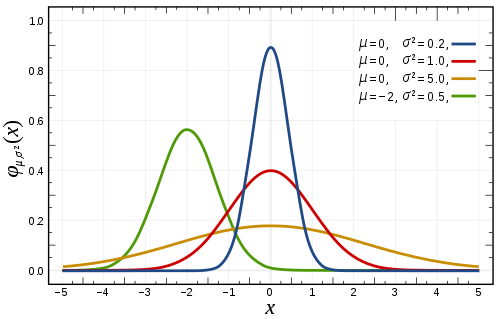
\includegraphics[width=0.46\textwidth]{img/normal}
      \caption{Quelle: Wikipedia}
\end{figure}
 \end{frame}



 \begin{frame}
    \frametitle{Erwartungswert}
\framesubtitle{}
\begin{block}{Beispiel}
Sei $X \sim \mathcal{N}(\mu, \sigma^2)$.
\begin{align*}
&\mathbb{V} (X) =  \frac{1}{\sqrt{2 \pi}} \int_{- \infty}^{\infty} x^2 e^{- \frac{x^2}{2}} \; dx =   \frac{1}{\sqrt{2 \pi}} \int_{- \infty}^{\infty} x (xe^{- \frac{x^2}{2}}) \; dx \\
& =  \frac{1}{\sqrt{2 \pi}} \biggl (\biggl [ x (e^{- \frac{x^2}{2}}) \biggr]_{- \infty}^{\infty}   - \int_{- \infty}^{\infty}  - e^{- \frac{x^2}{2}} \; dx  \biggr) = 0 + 1 = 1\\
\end{align*}
\href{https://de.wikipedia.org/wiki/Partielle_Integration}{LINK: Partielle Integration}. Mit "Verschiebungstrick"
$\Rightarrow \mathbb{V}(X) = \sigma^2$.
\end{block}
 \end{frame}



\begin{frame}
    \frametitle{Erwartungswert}
\framesubtitle{}
\begin{block}{Markov Ungleichung}
Sei $Y : \Omega \to \mathbb{R}$  eine  reelle, integrierbare  Zufallsvariable und $f : [0, \infty) \to [0, \infty)$ monoton wachsend.
Dann gilt für alle $\epsilon > 0$ mit $f(\epsilon) > 0$
\begin{align*}
P (|Y |  \geq \epsilon) \leq \frac{\mathbb{E} (f \circ |Y|)}{f(\epsilon)}
\end{align*}
\end{block}
\begin{block}{Beweis}
Da $f(\epsilon) 1_{\{ |Y| \geq  \epsilon \} } \leq f \circ |Y|$ folgt
\begin{align*}
f(\epsilon) P(|Y| \geq \epsilon) = & f(\epsilon) \mathbb{E}(1_{\{ |Y| \geq  \epsilon \} }) = \mathbb{E}( f(\epsilon) 1_{\{ |Y| \geq  \epsilon \} }) \\
\leq & \mathbb{E}( f \circ |Y|)
\end{align*}
\end{block}
 \end{frame}






\begin{frame}
    \frametitle{Erwartungswert}
\framesubtitle{}
\begin{block}{Tschebyscheff-Ungleichung}
Für eine reelle, integrierbare und quadratintegrierbare  Zufallsvariable $Y : \Omega \to \mathbb{R}$  gilt:
\begin{align*}
P (|Y  - \mathbb{E} (Y)|  \geq \epsilon) \leq \frac{\mathbb{V} (Y)}{ \epsilon^2} 
\end{align*}
\end{block}
\begin{block}{Beweis}
Folgt direkt aus der Markov-Ungleichung mit $Y' = Y -\mathbb{E}(Y)$ und $f(x) = x^2$
\end{block}
 \end{frame}



\begin{frame}
    \frametitle{Erwartungswert}
\framesubtitle{}
\begin{block}{Schwaches Gesetz der großen Zahlen}
Seien $X_i : \Omega \to \mathbb{R}$ unabhängige, reelle Zufallsvariablen (uiv, iid(englisch)) mit $\mathbb{E}(X_i) = \mu < \infty$ und $\mathbb{V}(X_i) = \sigma < \infty$, dann gilt
\begin{align*}
P \bigl  ( \bigl | \frac{1}{n} \sum_{i=1}^{n} X_i - \mu \bigr |  \geq \epsilon \bigr) \leq \frac{\sigma}{ n \cdot \epsilon^2} \; \; \underset{n \to \infty}{\longrightarrow} 0
\end{align*}
(stochastische Konvergenz). 
\end{block}
 \end{frame}


\begin{frame}
    \frametitle{Erwartungswert}
\framesubtitle{}
\begin{block}{Beweis}
Mit $Y_n =  \frac{1}{n} \sum_{i=1}^{n}  X_i - \mu$ ist $\mathbb{E}(Y_n) =  \frac{1}{n} \sum_{i=1}^{n} \mathbb{E}( X_i - \mu) = 0$ und 
$\mathbb{V}(Y_n) =  \frac{1}{n^2} \sum_{i=1}^{n} \mathbb{V}( X_i ) = \frac{\sigma}{n}$. Aus der Tschebyscheff-Ungleichung folgt die Behauptung.
\end{block}
 \end{frame}


\begin{frame}
    \frametitle{Erwartungswert}
\framesubtitle{}

\begin{figure}[htp]
      \centering
    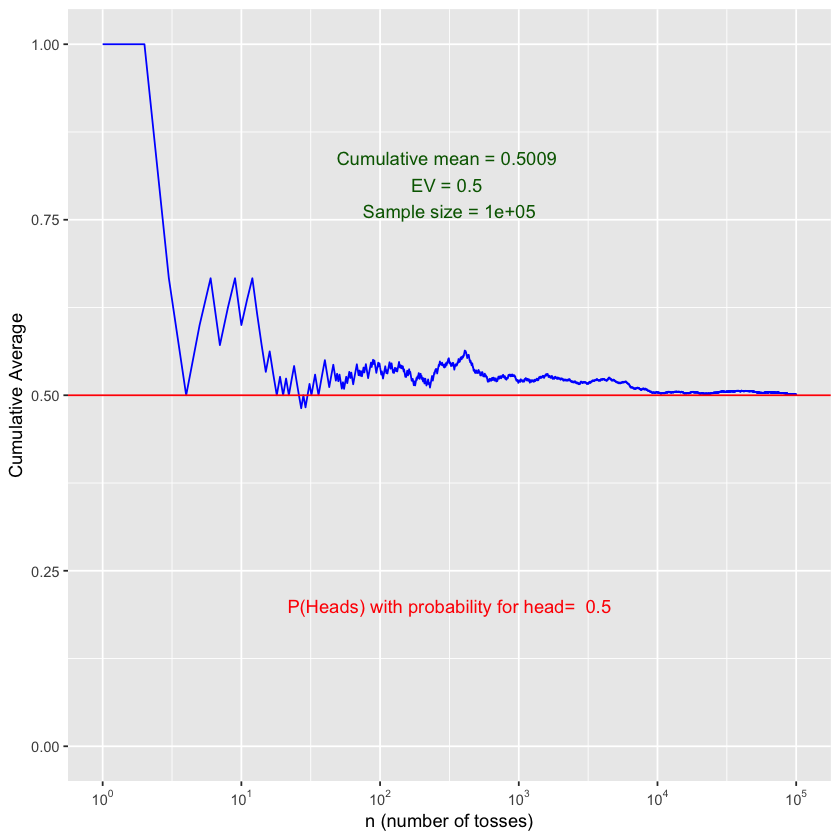
\includegraphics[width=0.86\textwidth]{img/sgdz}
      \caption{Quelle: Wikipedia}
\end{figure}
 \end{frame}


\end{document}
